This chapter contains a short summary of the concepts used in this thesis, and previous results this work is based upon, such as image moments, their relevance in image analysis, and more specifically Zernike moments and their state-of-the-art applications for both grayscale and color image analysis. Furthermore, some of the the most common use cases of image moments are provided.

\section{Image moments}
In general, image moments are certain descriptive values calculated using the pixel intensities of an image. Different moments can be used to extract certain properties from a picture, for example the centroid of a grayscale image can be calculated as
$$
\left\{ \overline{x}, \overline{y} \right\} = \left\{ \frac{M_{10}}{M_{00}},  \frac{M_{01}}{M_{00}} \right\},
$$ where $M_{ij}$ are the regular (geometric) image moments defined as
\begin{gather}
M_{ij} =  \sum_x \sum_y x^i y^j I(x,y) \label{eq:regular_moment},
\end{gather} with $I(x,y)$ being the pixel value at the coordinates $(x,y)$.

\subsection{Moment invariants}
Using specific image moments, so-called moment invariants can be defined, which are invariant under certain transformations, such as rotation, scaling, and translation.

These invariants are widely used in applications for pattern matching and image recognition~\cite{app1, app2, app3}. In particular, moment invariants can be used in medical applications, such as solving the Pathological Brain Detection problem~\cite{med_app_1}.

\section{Zernike moments}
Zernike functions, first introduced by Zernike~\cite{zernike} in 1934 are a system of complex, orthogonal polynomials defined on the unit disc. Using polar coordinates the Zernike polynomials $V_{n,m}$ ($n \in \mathds{N}$, $m \in \mathds{Z}$, $n \geq |m|$ and $n - |m|$ is even) are defined as
\begin{gather*}
  V_{n,m}(r,\theta) = R_{n,m}(r) e^{i m\theta},
\end{gather*}
where $ R_{n,m}(r) $ are the radial polynomials defined as
\begin{gather}
  R_{n,m}(r) = \sum_{k=0}^{\frac{n - |m|}{2}}\frac{(-1)^k (n - k)!}{k!\left(\frac{n + |m|}{2} - k\right)!\left(\frac{n - |m|}{2} - k\right)!}r^{n-2k} \label{eq:radial_poly}.
\end{gather}

It is important to note that these radial polynomials are the same for $m$ and $-m$, and satisfy an orthogonality relation over $[0,1]$ with respect to the weight $r$ (see e.g. \cite{schipp}), i.e. for a fixed $m$ we have
\begin{equation}\label{Rortho}
	\int_0^1 R_{n,|m|}(r) R_{n',|m|}(r)r\ dr  = \frac{1}{2n+2} \delta_{n,n'},
\end{equation}
and can be expressed in terms of the shifted Jacobi polynomials in the following way:
\begin{equation}\label{RJacobi}
	R_{n,m}(r) = r^{|m|} P_{\frac{n - |m|}{2}}^{(0,|m|)}(2r^2-1),
\end{equation}
where we denoted the $k$-th degree classical Jacobi polynomials by $P_k^{(\alpha,\beta)}$ (see e.g. \cite{Szego}).


Zernike moments are image moments, defined for grayscale images inside the unit circle, using the Zernike polynomials.
The system of Zernike polynomials proved to be a suitable basis for series expansions in numerous optical applications (see for example~\cite{wavefront,optical_human_eye,opt_surf}), and moment invariants could easily be constructed using the Zernike moments~\cite{zernike_moments}. 

The Zernike moment of order $n$ and repetition $m$ of a grayscale, continuous image function $f(r,\theta)$ given in polar coordinates is defined as
\begin{gather*}
  Z_{n,m}(f) = \frac{n + 1}{\pi}\int_0^1\int_0^{2\pi}f(r,\theta)V_{n,m}^{*}(r,\theta)r\ dr\ d\theta.
\end{gather*}

Since the Zernike polynomials are orthogonal, the following approximate reconstruction of the image function is possible, using Zernike moments only up to a finite $M$ degree:

\begin{gather*}
  f(r,\theta) \approx \sum_{n=0}^{M}\sum_{m=-n}^{n}Z_{n,m}(f)V_{n,m}(r,\theta).
\end{gather*}

Since digital images are not represented in polar coordinates and are not defined only over the unit disc, a transformation of the image onto the unit disk is needed. The most commonly used transformation is a linear transformation from the image coordinates to a suitable square inside the unit circle. This transformation is described in more detail in Section~\ref{sec:discretization}.
After the linear transformation, the following discrete approximation can be used to calculate the Zernike moments of a digital image $f(x,y)$
\begin{gather*}
  Z_{n,m}(f) = \frac{2(n+1)}{\pi(N-1)^2}\sum_{x=1}^{N}\sum_{y=1}^{N}f(x,y)V_{n,m}^{*}(r_{x,y},\theta_{x,y}),
\end{gather*}
where $N$ is the size of the image, and $(r_{x,y},\theta_{x,y})$ are the polar coordinates corresponding to the $(x,y)$ image coordinates.

\section{Quaternions and color image moments}
The previously defined Zernike moments can only be used for grayscale images, and extending signal processing techniques efficiently to multichannel color images is an important and generally unresolved problem.

Conventionally, for multichannel, color images, two main approaches are being used. Either the image is converted to grayscale so that the moments defined for grayscale images could be used, or (after RGB-decomposition) the grayscale method is used on each channel of the image~\cite{affine_color}.

More recently, the algebra of quaternions was employed to various conventional moments so that color images can be analysed holistically.

\subsection{Quaternion representation of color images}

A quaternion, $q$, was defined by \citeauthor{Hamilton} \cite{Hamilton} as a generalization of the complex numbers: 
\[
	q = a+b\qi +c\qj+d\qk.
\]
The real numbers $a , b , c$ and $d$ are called the components of $q$ , and the imaginary units $\qi , \qj, \qk$ are defined according to the following rules:
\[
\begin{gathered}
	\qi^2 = \qj^2 = \qk^2 = \qi\qj\qk = -1,\\
	\qi\qj = -\qj\qi = \qk,\ \qj\qk = -\qk\qj = \qi,\ \qk\qi = -\qi\qk = \qj.
\end{gathered}
\]

Therefore, the set of quaternions $\Hq$ is an \textit{algebra}, where a quaternion is called pure quaternion when $a=0$. 
The conjugate and modulus of $q$ are respectively defined by 
\[
\begin{gathered}
q^* = a-b\qi-c\qj-d\qk, \\
|q| = \sqrt{a^2+b^2+c^2+d^2}.
\end{gathered}
\]

\citeauthor{EllSangwine} \cite{EllSangwine} utilized quaternions to represent a color image, $f: \R^2\to\R^3$ , as follows:
\[
f(x,y) = \qi f_R(x,y) + \qj f_G(x,y) + \qk f_B(x,y),
\]
where functions $f_R , f_G, f_B:\R^2\to\R$ represent the red, green and blue components of the $(x,y)$ pixel, respectively.

% Quaternions are a generalization of complex numbers, consisting of one real and three imaginary parts. A quaternion $q$ can be represented in the form $q = a + b\mathbf{i} + c\mathbf{j} + d\mathbf{k}$, where $a,b,c,d \in \mathds{R}$ and $\mathbf{i}, \mathbf{j}, \mathbf{k}$ are the imaginary units, defined by the multiplication rules $\mathbf{i}^2 = \mathbf{j}^2 = \mathbf{k}^2 = \mathbf{ijk} = -1$. The set of quaternions is denoted by $\mathds{H}$.

For example, \citeauthor{qfmm}~\cite{qfmm} introduced quaternion Fourier-Mellin moments (QFMMs) which are an extension of the conventional Fourier-Mellin moments. Similarly, the same quaternion techniques were applied successfully to other function systems (e.g.~\cite{bessel-fourier, chebyshev-fourier}), yielding similar results.

% The main idea behind these extensions is that an RGB image can be viewed as a pure quaternion valued function, with each color component corresponding to one of the imaginary units.

\subsection{Quaternion Zernike moments}\label{sec:qzm}
\citeauthor{qzm}~\cite{qzm,qzmi} proposed the quaternion Zernike moments (QZMs), an extension of conventional Zernike moments to color images using quaternions. Generally, this method overperforms other similar approaches in color image recognition, due to the natural invariances of Zernike functions.

Quaternion Zernike moments, just as regular Zernike moments, are defined over the complex unit disk
\[
	\D = \left\{ z = re^{i\theta}\in\C \ :\ r\in[0,1],\theta\in[0,2\pi)\right\}.
\]

The main difference, compared to the conventional Zernike moments is that instead of the complex-valued Zernike functions, QZMs use a quaternion-valued generalization of the Zernike functions as a basis for the series expansion. The quaternion generalizations of classical Zernike functions, defined as 
\[
	\phi_{n,m}(r,\theta) = R_{n,m}(r) e^{-\qmu m\theta},
\]
satisfy the orthogonality relation
\begin{equation}\label{QZortho}
	\frac{n+1}{\pi} \int_0^1 \int_0^{2\pi} \phi_{n,m}(r,\theta) \phi^*_{n',m'}(r,\theta) r \ d\theta dr = \delta_{n,n'}\delta_{m,m'}.
\end{equation}

Let $f(r,\theta)$ be a pure quaternion valued, RGB image function with a continuous domain, defined in polar coordinates on the unit circle $\D$. Each color component corresponds to one of the imaginary units. Let $\bm{\mu} = \frac{\mathbf{i} + \mathbf{j} + \mathbf{k}}{\sqrt{3}}$ be a unit pure quaternion.

Since the multiplication of quaternions is not commutative, both right-side and left-side quaternion Zernike moments can be defined. The right-side QZM of order $n$ and repetition $m$ is defined as
\begin{gather}
  \begin{split}
  Z_{n,m}^R(f) &= \frac{n + 1}{\pi}\int_0^1\int_0^{2\pi}R_{n,m}(r)f(r,\theta)e^{-\bm{\mu}m\theta}r\ dr\ d\theta, \\
  &n \geq |m| \text{  and  } n - |m| \text{  is even.}
  \end{split}
  \label{eq:QZRM}
\end{gather}

The left-side QZMs are defined as 
\begin{gather*}
  Z_{n,m}^L(f) = \frac{n + 1}{\pi}\int_0^1\int_0^{2\pi}R_{n,m}(r)e^{-\bm{\mu}m\theta}f(r,\theta)r\ dr\ d\theta.
\end{gather*}

Similarly to non-quaternion Zernike moments, the original image can be approximated by using either right-side or left-side QZMs only up to a finite $M$ degree.
\begin{gather}
\begin{split}
  f(r,\theta) &\approx \sum_{n=0}^{M}\sum_{m=-n}^{n}Z_{n,m}^R(f)R_{n,m}(r)e^{\bm{\mu}m\theta} \\
  f(r,\theta) &\approx \sum_{n=0}^{M}\sum_{m=-n}^{n}e^{\bm{\mu}m\theta}Z_{n,m}^L(f)R_{n,m}(r)
\end{split}\label{eq:qzm_reconstruction}
\end{gather}

In this thesis, only the right-side QZMs will be used, because of the following relation between right- and left-side QZMs:
\begin{gather*}
  Z_{n,m}^L(f) = -(Z_{n,m}^R(f))^{*}
\end{gather*}

The discretization of the QZMs and the transformation of arbitrary digital RGB images onto the unit disk is described in detail in Section~\ref{sec:discretization} 

\section{Discretization of QZMs}\label{sec:discretization}
The conventional Zernike moments and the QZMs are defined in terms of polar coordinates, for image functions, whose domain is the unit disk. On the other hand, digital images are usually defined in image coordinates, with the coordinates being integers ranging from $0$ to $N - 1$ (the number of pixels along each axis).

There are two "natural" ways to linearly transform a square image from image coordinates to polar coordinates inside the unit circle, using only translation and scaling~\cite{kintner}.

The first method is to transform the entire image inside the unit circle, as shown on Figure~\ref{fig:transform1}. This way all of the pixels will be used for calculating the (quaternion) Zernike moments, but some areas of the unit disk will remain empty, no pixels fall on those areas.

The other method is to transform the image such that the unit disk becomes the inscribed circle of the square image, as shown on Figure~\ref{fig:transform2}. This method fills the entire unit disk with pixels, but some pixels fall outside the unit cirle and thus will not be used for the calculation of (quaternion) Zernike moments.

The polar coordinates $(r,\theta)$ corresponding to the image coordinates $(x,y)$ can be calculated by the following formulas, which is the mapping proposed by \citeauthor{Chong}~\cite{Chong}:
\begin{gather*}
  r = \sqrt{(c_1x + c_2)^2 + (c_1y + c_2)^2}, \\
  \theta = \tan^{-1}\left(\frac{c_1y + c_2}{c_1x + c_2}\right),
\end{gather*}
where $c_1$, $c_2 \in \mathds{R}$ depend on which of the previously mentioned transformations is used. A $\lambda \in \mathds{R}$ scaling factor is also defined for each transformation.
For the first one (Figure~\ref{fig:transform1}): $c_1 = \frac{\sqrt{2}}{N - 1}$, $c_2 = -\frac{1}{\sqrt{2}}$, and $\lambda = \frac{2}{\pi}$. While for the other transformation (Figure~\ref{fig:transform2}): $c_1 = \frac{2}{N - 1}$, $c_2 = -1$ and $\lambda = 1$.

\begin{figure}[tb]
  \begin{subfigure}{.43\textwidth}
  \centering
    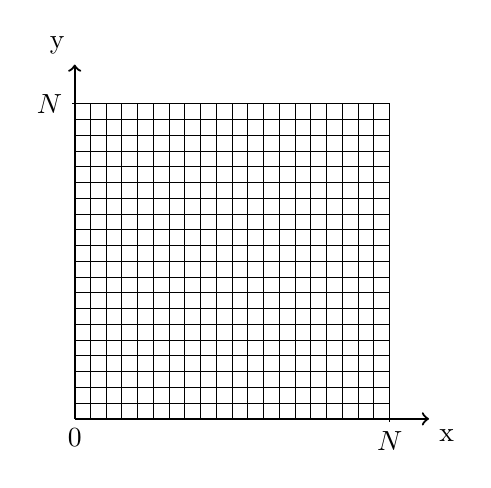
\begin{tikzpicture}
      \draw[step=0.2cm,black] (0,0) grid (4,4);
      \draw[thick,->] (0,0) -- (4.5,0) node[anchor=north west] {x};
      \draw[thick,->] (0,0) -- (0,4.5) node[anchor=south east] {y};
      \draw (4cm,1pt) -- (4cm,-1pt) node[anchor=north] {$N$};
      \draw (1pt,4cm) -- (-1pt,4cm) node[anchor=east] {$N$};
      \draw (0,0) -- (0,0) node[anchor=north] {$0$};
    \end{tikzpicture}
  \caption{An $N \times N$ image on the image plane}
  \end{subfigure}
  \begin{subfigure}{.05\textwidth}
    \centering
    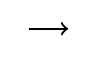
\begin{tikzpicture}
      \draw[thick,->] (0,0) -- (0.5,0);
    \end{tikzpicture}
  \end{subfigure}
  \begin{subfigure}{.50\textwidth}
    \centering
      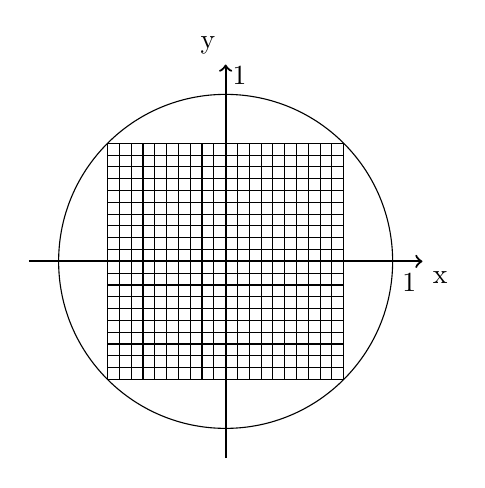
\begin{tikzpicture}
        \draw[step=0.15cm,black] (-1.5,-1.5) grid (1.5,1.5);
        \draw[thick,->] (-2.5,0) -- (2.5,0) node[anchor=north west] {x};
        \draw[thick,->] (0,-2.5) -- (0,2.5) node[anchor=south east] {y};
        \draw (0,0) circle (2.121cm);
        \draw (2.121cm,1pt) -- (2.121cm,-1pt) node[anchor=north west] {$1$};
        \draw (1pt,2.121cm) -- (-1pt,2.121cm) node[anchor=south west] {$1$};
      \end{tikzpicture}
    \caption{The image transformed inside the unit circle}
    \end{subfigure}
  \caption{The image before and after applying the transformation inside the unit disk}
  \label{fig:transform1}
\end{figure}

\begin{figure}[tb]
  \begin{subfigure}{.43\textwidth}
  \centering
    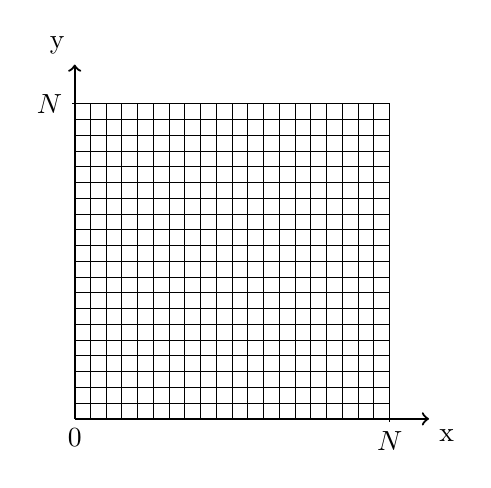
\begin{tikzpicture}
      \draw[step=0.2cm,black] (0,0) grid (4,4);
      \draw[thick,->] (0,0) -- (4.5,0) node[anchor=north west] {x};
      \draw[thick,->] (0,0) -- (0,4.5) node[anchor=south east] {y};
      \draw (4cm,1pt) -- (4cm,-1pt) node[anchor=north] {$N$};
      \draw (1pt,4cm) -- (-1pt,4cm) node[anchor=east] {$N$};
      \draw (0,0) -- (0,0) node[anchor=north] {$0$};
    \end{tikzpicture}
  \caption{An $N \times N$ image on the image plane}
  \end{subfigure}
  \begin{subfigure}{.05\textwidth}
    \centering
    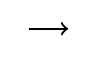
\begin{tikzpicture}
      \draw[thick,->] (0,0) -- (0.5,0);
    \end{tikzpicture}
  \end{subfigure}
  \begin{subfigure}{.50\textwidth}
    \centering
      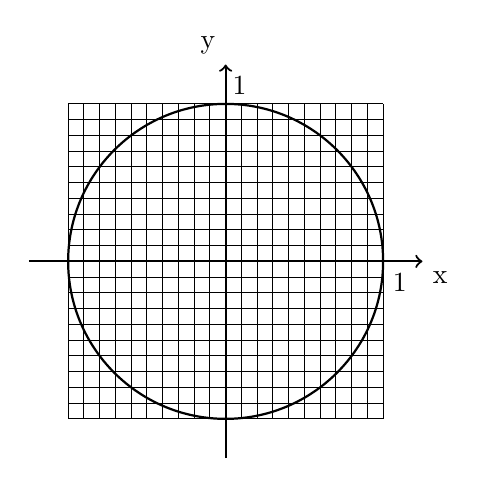
\begin{tikzpicture}
        \draw[thin,step=0.2cm,black] (-2,-2) grid (2,2);
        \draw[thick,->] (-2.5,0) -- (2.5,0) node[anchor=north west] {x};
        \draw[thick,->] (0,-2.5) -- (0,2.5) node[anchor=south east] {y};
        \draw[thick] (0,0) circle (2cm);
        \draw (2cm,1pt) -- (2cm,-1pt) node[anchor=north west] {$1$};
        \draw (1pt,2cm) -- (-1pt,2cm) node[anchor=south west] {$1$};
      \end{tikzpicture}
    \caption{The image transformed onto the unit disk}
    \end{subfigure}
  \caption{The image before and after applying the transformation onto the unit disk}
  \label{fig:transform2}
\end{figure}

In general, using the polar form of the transformed coordinates, the continuous integral of \eqref{eq:QZRM} can be replaced by discrete approximations of form
\begin{equation}\label{eq:QZMappr}
	Z_{n,m}^R(f) \approx \lambda_{n,m} \sum_{k=1}^{N_1} \sum_{j=1}^{N_2} f(r_k,\theta_j) \phi(r_k,\theta_j) w(r_k,\theta_j),
\end{equation}
with some discretization weight function $w$ and normalization constants $\lambda_{n,m}$.

Using either one of the previously defined transformations, a points system on the unit disk is obtained, and for each point exactly one pixel value is assigned. When this points system is used for the discretization of QZMs, the following formula can be used to approximate the QZMs of the original image function:
\begin{gather*}
  Z_{n,m}^R(f) \approx \lambda\frac{n + 1}{(N - 1)^2}\sum_{x = 0}^{N-1}\sum_{y = 0}^{N-1}R_{n,m}(r_{x,y})f(x,y)e^{-\bm{\mu}m\theta_{x,y}},
\end{gather*}
where $f \in \mathds{R}^2 \rightarrow \mathds{H}$ is the RGB image defined in image coordinates, $(r_{x,y},\theta_{x,y})$ are the polar coordinates belonging to the image coordinates $(x,y)$, and $\lambda$ is the previously defined scaling factor.

In the rest of this thesis, for comparison purposes, the transformation of the image inside the unit circle will be used as \citeauthor{qzmi}~\cite{qzmi} used this discretization to present their results.

\subsection{Other approaches for discretization}
A similar approach was utilized numerous times in the literature, substituting the radial polynomial system $R_{n,m}$ of Zernike functions with other well-known orthogonal systems over the radial interval $[0,1]$. For color image analysis, further examples of this include the QFMMs \cite{qfmm}, the QPETs, QPCTs and QPSTs \cite{Li}, the QCMs \cite{Guo}, the QBFMs \cite{Shao}, the QRHFMs \cite{Wang}, the QG-CHFMs and QG-PJFMs \cite{Singh} and the QSBFMs \cite{Yang}.

This natural method was proven susceptible to inaccuracies of both geometric and numeric nature when applied to grayscale images (see e.g.  \cite{LiaoPawlak}, \cite{PawlakLiao}), and these problems are carried over to the quaternion generalizations as well. Later in \cite{Xin}, a more accurate computational technique was proposed, where $\D$ is partitioned into polar sectors of approximately equal areas, and the original pixels are transformed to the centroids of these via cubic interpolation, and the weights are computed by performing the integration of functions $\phi_{n,m}$ over the respective polar sectors.

The same idea, adapted to quaternion-type moments for any aforementioned radial system, could substantially improve performances for tasks like image reconstruction, as well as recognition after rotation, scaling and translation (RST) transformations and addition of different kinds of noise; and the reason for this is essentially the improved accuracy gained for the computation of respective moments and invariants. Examples of this technique applied for color images include the papers of \citeauthor{HosnyLegendre} for Legendre \cite{HosnyLegendre} and Chebyshev \cite{HosnyChebyshev} radial systems.

A drawback of this approach is that the cubic interpolation applied for coordinate transformation is irreversible, so another transformation with further introduced error is required if one wishes to reconstruct the original square/rectangle shaped image. Instead, in the previous works \cite{LiaoPawlak,PawlakLiao,Xin,HosnyLegendre,HosnyChebyshev}, reconstruction error was measured for the transformed image and its reconstructions on disc $\D$ only. Another, although minor issue is the natural smoothing provided by the cubic interpolation, which unintentionally improves the obtained results for experiments on noisy images by filtering some of the noise, a sometimes unwanted side effect for one who wants to compare the performances of the moments themselves. To ensure fair comparisons with the first transformation group, linear interpolation should be used, ensuring invertible coordinate transformations, and also excluding unwanted side effects.

Finally, the results of \citeauthor{WangAcc} \cite{WangAcc} and \citeauthor{LiuAcc} \cite{LiuAcc} for radial harmonic Fourier moments are some of the recent advances in the study of quaternion moments, introducing a novel coordinate transformation, which seems to improve accuracy for this specific function system while maintaining fast computation times, without utilizing cubic interpolation at all. These improvements may seem surprising at first, but hopefully our results will clarify the theoretical reason behind them.

\subsection{Discrete orthogonality}
Even though the Zernike polynomials are a set of orthogonal polynomials on the complex unit disk, the previously defined points systems do not provide discrete orthogonality. 
This is problematic, and results in poor performances especially for applications under noisy conditions.
Also, the lack of orthogonality makes the moment representation of an image redundant, hence introducing unwanted reconstruction errors.

\section{Quaternion Zernike Moment Invariants (QZMIs)}\label{sec:invariance}
\citeauthor{qzmi}~\cite{qzm, qzmi} proposed the constructions described in this section in order to create rotation, scaling and translation invariant moment invariants using the quaternion Zernike moments.

\subsection{Translation invariance}
In order to achieve translation invariance, the common centroid of all three color channels can be calculated by using zero-order and first-order geometric moments, as described by \citeauthor{affine_color}~\cite{affine_color}.
If the origin of the polar coordinate system is placed on this common centroid $(x_c, y_c)$, then the QZMs calculated in this coordinate system will be translation invariant. Let $\overline{Z}_{n,m}^R(f)$ denote the translation invariant QZMs.

\subsection{Rotation invariance}
To achieve rotation invariance consider the image rotated by some degree $\alpha$: $f'(r,\theta) = f(r, \theta - \alpha)$. \citeauthor{qzmi}~\cite{qzmi} proved that for the rotated image $Z_{n,m}^R(f') = Z_{n,m}^R(f)e^{-\bm{\mu}m\theta}$ and $Z_{n,m}^L(f') = e^{-\bm{\mu}m\theta}Z_{n,m}^L(f)$. Because of the these properties 
$$\Phi_{n,k}^m = Z_{n,m}^R(f)Z_{k,-m}^L(f) = -Z_{n,m}^R(f)(Z_{k,m}^R(f))^*$$
is invariant to rotation. In the following chapters, this will be referred to as a quaternon Zernike moment rotation invariant (QZMRI).

Previously, the modulus $|Z_{n,m}^R(f)|$ was used to achieve rotation invariance~\cite{qzm}, but this provided only one real-valued invariant, whereas the following construction provides a quaternion-values invariant.

\subsection{Scaling invariance}
For non-negative integers $m$ and $l$, \citeauthor{qzmi}~\cite{qzmi} constructed the following scaling invariants utilizing the symmetric property of the radial polynomials with respect to $m$ and an alternate form of the QZMs.

\begin{gather*}
  \begin{split}
  c_{m,l}^{t,k} &= (-1)^{l-k}\frac{(m + 2l + 1)(m + k + l)!}{(l - k)!(k - t)!(m + k + t + 1)!} \\
  L_{m + 2l,m}^R(f) &= \sum_{t=0}^l\sum_{k=t}^l\left(\sqrt{|Z_{0,0}^R(f)|}\right)^{-(m+2k+2)}c_{m,l}^{t,k}Z_{m+2t,m}^R(f).
  \end{split}
\end{gather*}

\subsection{Combined RST invariance}
Similarly to using QZMs to define rotation invariants, the previously defined scaling invariants can also be used to construct $\Psi_{n,k}^m = L_{n,m}^R(f)(L_{k,m}^R(f))^*$, which is invariant to rotation and scaling.

In order to achieve translation invariance, throughout the construction of the scaling invariants $L_{n,m}^R$ the translation invariant QZMs ($\overline{Z}_{n,m}^R(f)$) can be used, thus defining the $\overline{L}_{n,m}^R$ translation and scaling invariants.

Furthermore, $\overline{\Psi}_{n,k}^m = \overline{L}_{n,m}^R(f)(\overline{L}_{k,m}^R(f))^*$ is invariant to rotation, scaling and translation~\cite{qzmi}. This is called a quaternion Zernike moment invariant (QZMI).

\section{Applications}
Zernike moments and moment invariants are a useful tool in optical and medical applications. Specifically, Zernike moments can be used in the representation of optical aberration~\cite{wavefront,optical_human_eye,opt_surf}.

Furthermore, applications in pattern recognition have shown that in noisy environments Zernike moment yield the best results~\cite{pattern_recognition}. \citeauthor{hand_vein}~\cite{hand_vein} have used Zernike moment invariants to extract descriptions of hand vein patterns.

Another application is in image watermarking so that the watermark is invariant to transformations and robust against noise~\cite{watermarking_auth, robust_watermarking, invariant_watermark}.

Finally, one possible application is to use Zernike moments in conjunction with neural networks. The robustness of neural networks with respect to noise is a known shortcoming of current systems~\cite{nn_robust,nn_noise_robust}. Zernike moments can be used to extract features of images with high robustness to noise, so these extracted features can be used as input for neural networks~\cite{zernike_nn,zernike_nn2}. 